% !TEX TS-program = pdflatex
% !TEX encoding = UTF-8 Unicode

% This file is a template using the "beamer" package to create slides for a talk or presentation
% - Giving a talk on some subject.
% - The talk is between 15min and 45min long.
% - Style is ornate.

% MODIFIED by Jonathan Kew, 2008-07-06
% The header comments and encoding in this file were modified for inclusion with TeXworks.
% The content is otherwise unchanged from the original distributed with the beamer package.


% http://tex.stackexchange.com/questions/99049/latex-error-option-clash-for-package-xcolor-even-if-i-put-listings-before
\PassOptionsToPackage{usenames,dvipsnames}{xcolor}

\documentclass{beamer}

% Copyright 2004 by Till Tantau <tantau@users.sourceforge.net>.
%
% In principle, this file can be redistributed and/or modified under
% the terms of the GNU Public License, version 2.
%
% However, this file is supposed to be a template to be modified
% for your own needs. For this reason, if you use this file as a
% template and not specifically distribute it as part of a another
% package/program, I grant the extra permission to freely copy and
% modify this file as you see fit and even to delete this copyright
% notice. 

\mode<presentation>
{
  \usetheme{boxes}
  \usecolortheme{beaver}
  \setbeamercovered{transparent}
  % or whatever (possibly just delete it)
}

\usepackage[english]{babel}

\usepackage{parskip}
\usepackage{tikz}
\usetikzlibrary{arrows,matrix,decorations.markings,decorations.pathreplacing}
% Bigger arrowheads
\tikzset{
  big arrow/.style={
    decoration={markings,mark=at position 1 with {\arrow[scale=2,#1]{>}}},
    postaction={decorate},
    shorten >=0.4pt},
  big arrow/.default=black}
  
\usepackage{amsopn}
\DeclareMathOperator{\Hom}{Hom}


\usepackage[utf8]{inputenc}

\usepackage{times}
\usepackage[T1]{fontenc}
% Or whatever. Note that the encoding and the font should match. If T1
% does not look nice, try deleting the line with the fontenc.

\usepackage{subfig}
\usepackage{graphicx,multicol}
\usepackage{siunitx}


\title[Vector Bundles] % (optional, use only with long paper titles)
{Vector Bundles}

\subtitle{or What is a Tensor?}

\author{Lorne Whiteway \\ lorne.whiteway@star.ucl.ac.uk}
\date{31 January \& 7 February 2017}

% If you wish to uncover everything in a step-wise fashion, uncomment
% the following command: 
%\beamerdefaultoverlayspecification{<+->}

\begin{document}

% See https://tex.stackexchange.com/questions/82456/how-to-remove-figure-caption-prefix-figure-in-beamer
\setbeamertemplate{caption}{\raggedright\insertcaption\par}

\begin{frame}
  \titlepage
\end{frame}

\section{Introduction}

\begin{frame}{Exercise 1}
Show that there must be some date during the year where the historical average temperature on that date is the same as the historical average temperature six months later.

This result is related to the circular topology ($S^1$) of the set of dates.
\end{frame}

\begin{frame}{Exercise 2}
Consider the coordinate transformation:
\begin{equation*}
x'_1 = \frac{x_1}{x_1^2 + x_2^2} \hspace{1cm} x'_2 = \frac{x_2}{x_1^2 + x_2^2} \hspace{1cm} \text{where} \hspace{0.5cm} x_1^2 + x_2^2 \neq 0
\end{equation*}

What's the geometry of this space?

The coordinate description is crucial for calculations but doesn't always give geometrical intuition. The goal of this talk is to re-express the tensors of General Relativity in a way that makes the geometry clear.

\end{frame}

\begin{frame}{Where We are Going}

I begin with some examples to motivate looking at \textit{parameterised families of vector spaces} (i.e. \textit{vector bundles}).

\end{frame}

\begin{frame}{Graphs of Functions}

We write $f \colon X \to Y$ to denote a function taking elements of $X$ (the \textit{domain}) to elements of $Y$ (the \textit{range}). The \textit{graph} of f is then a subspace of $X \times Y$.

Let $I$ denote an interval of the real line (e.g. $[0, 1]$). Most graphs that appear in journals are of the form $f \colon I \to I$ as these are easy to print!

Of course we can have arbitrary topology for both the domain and the range:
\begin{equation*}
\begin{split}
\text{CMB temperature } \colon S^2 \to \mathbb{R} \\
\text{Time of day} \colon \mathbb{R} \to S^1
\end{split}
\end{equation*}

\end{frame}

\begin{frame}{Different Range for each Point in the Domain?}

Consider the vertical displacement to the Earth's surface caused by an earthquake. This is a mapping $D \colon S^2 \to  \mathbb{R}^3$.

But we know that at any point $p$, $D(p)$ will lie in a particular one-dimensional subspace of $\mathbb{R}^3$ - namely the line normal to the surface at $p$.

Generalise this example to consider functions with a \textit{different range for each point in the domain}.

\end{frame}

\begin{frame}{Wind}

As another example consider the wind vector at each point on the Earth's surface. (Assume that wind is horizontal and that the wind field is continuous.)

This is a mapping $W \colon S^2 \to \mathbb{R}^3$.

However we know that each $W(p)$ lies in a particular subspace of $\mathbb{R}^3$ namely the tangent plane $T_p(S^2)$ to $S^2$ at $p$.

 Note that each tangent plane is different (almost: the tangent planes at $p$ and its antipode are the same subspace of $\mathbb{R}^3$).

\end{frame}


\begin{frame}{Vector Spaces}

Abstract vector spaces generalise the geometric picture of $\mathbb{R}^n$ and its linear subspaces.

They arise in any situation in which addition and multiplication by scalars are defined, satisfy the obvious axioms, and result in elements within the same set.

Examples:
\begin{itemize}
\item{elements $(x_1, x_2, x_3)$ satisfying $3x_1 + 5x_2 - 4x_3 = 0$}
\item{degree five polynomials $p$ satisfying $p(3)=0$}
\item{solutions $f$ to the linear differential equation $Df=0$}

\end{itemize}

\end{frame}


\begin{frame}{Mental Pictures}

- What's your mental picture of a vector space?

Remember most vector spaces don't have canonically defined axes. But they do all have a well-defined zero point.

- What's your mental picture of a vector?

Mathematicians think of a vector $v$ as simply a point in the vector space. Physicists tend to draw an arrow from $0$ to $v$. The pictures are interchangeable.

\end{frame}



\begin{frame}{So What's This a Picture Of?}
\begin{figure}
\begin{center}
\begin{tikzpicture}
\path[draw,big arrow] (4,0) -- (5,2);
\path[draw,big arrow] (8,1) -- (11,-1);
\end{tikzpicture}
\end{center}
\end{figure}

\end{frame}


\begin{frame}{A Vector Space at Each Point}

The two vectors in the previous picture are in different vector spaces (they must be different as they have different zero points). Presumably there is a vector space anchored to each point in the plane, and we are seeing examples of vectors in two of those vector spaces.

\end{frame}


\begin{frame}{Vector Bundles}

A \textit{vector bundle} $B$ is a parameterised family of vector spaces, one (call it $B_p$) for each point $p$ in some parameter space $P$.

All the vector spaces in the bundle must have the same dimension.

If $a$ and $b$ are nearby in $P$ then the vector spaces $B_a$ and $B_b$ must also be nearby (in a sense that we could make precise).


\end{frame}


\begin{frame}{Topology, but No Metric}

In this talk I assume \textit{topological} structure but not \textit{metric} structure.

You can count holes but you can't measure distances. You can stretch but you can't rip or tear or puncture. Donuts equal coffee mugs.

The concept `nearby' can actually be made precise (but not by using a quantitative measure of distance).

\end{frame}


\begin{frame}{Parameter Spaces are Manifolds}

Our parameter spaces are \textit{manifolds} i.e. geometrical spaces that topological locally (but not necessarily globally) look like $\mathbb{R}^n$.

Examples:
\begin{itemize}
\item{$S^1$, $S^2$, $S^n$}
\item{$T = S^1 \times S^1 = \text{torus}$}
\item{$RP^2 = \text{projective plane}$}
\item{Spacetime}
 \end{itemize}

\end{frame}


\begin{frame}{Terminology}

The union of all vector spaces in the bundle is the \textit{total space}.

The parameter space is called the \textit{base}.

The vector space $B_p$ may also be called the \textit{fibre} above $p$ (think of a shag carpet).

A continuous function $s$ that assigns to each point $p$ in the parameter space a vector $s(p)$ that lies in $B_p$ is called a \textit{cross-section} (again think of a shag carpet) or simply a \textit{section}.

The set of all sections is denoted $H^0(P, B)$.

\end{frame}

\begin{frame}{Example - Lines Bundles on $S^1$}

A bundle with one-dimensional fibres is called a \textit{line bundle}.

Let's look at some line bundles over the circle $S^1$.

\end{frame}

\begin{frame}{Example - Normal Bundle on $S^1$}

Consider $p=(x, y)$ in $S^1$ (so $x^2+y^2=1$).

 Let $N_p$ be the one-dimensional subspace of $\mathbb{R}^2$ consisting of all multiples of $(x,y)$.
 
 Then $N$ is the \textit{normal} bundle over $S^1$.

\end{frame}

\begin{frame}{Example - Tangent Bundle on $S^1$}

Consider $p=(x, y)$ in $S^1$ (so $x^2+y^2=1$).

Let $T_p$ be the one-dimensional subspace of $\mathbb{R}^2$ consisting of all multiples of $(y,-x)$.
 
Then $T$ is the \textit{tangent} bundle over $S^1$.

\end{frame}

\begin{frame}{Example - Constant Bundle on $S^1$}

Let $V$ be a one-dimensional vector space (e.g. $\mathbb{R}^1$).

Let $C_p$ be $V$ (for all $p$ in $S^1$).
 
Then $C$ is the \textit{constant} bundle (with fibre $V$) over $S^1$.

\end{frame}


\begin{frame}{Example - `Twisted' Bundle on $S^1$}

Consider $p=\exp{(i \theta)}$ in $S^1$.

Let $M_p$ be the one-dimensional subspace of $\mathbb{R}^2$ consisting of all multiples of $\exp{(i \theta /2)}$.

Note that this `works OK' in that we get back to where we started after going around the circle.
 
Then $M$ is the \textit{`twisted'} bundle over $S^1$.

\end{frame}

\begin{frame}{Example - Tangent Bundle to $S^2$}

The fibre at each point is the two dimensional subspace of $\mathbb{R}^3$ that is (parallel to) the tangent plane to the sphere at that point.

The total space is thus $2 + 2 = 4 \text{ dimensional}$ - hard to visualise!

\end{frame}


\begin{frame}{Tangent Bundle in General}

For each manifold $M$ we can build a vector bundle - the \textit{tangent bundle $TM$} - with tangent spaces as fibres.

If the manifold has dimension $n$ then so does each tangent plane so the total space has dimensionality $2n$.

Section of the tangent bundle  = vector field.

[We can do this construction even if the manifold is defined abstractly i.e. not simply given as a subset of $\mathbb{R}^n$. For this we need the manifold to have a \textit{differentiable structure} (intermediate between topology and a metric).]



\end{frame}

\begin{frame}{Equality of Vector Bundles}

Two vector bundles $B$ and $C$ over $M$ are \textit{isomorphic} (i.e. considered to be the same) if there is a family of vector space isomorphisms $f_p \colon B_p \to C_p$ that varies continuously with $p$.

Recall that a \textit{vector space isomorphism} is simply an invertible linear map.

\end{frame}

\begin{frame}{Trivial Bundles}

A bundle is \textit{trivial} if it is isomorphic to the constant bundle $M \times \mathbb{R}^n$ (i.e. where every fibre is just $\mathbb{R}^n$).

This is equivalent to having $n$ sections that are linearly independent at each point.

\end{frame}

\begin{frame}{Exercise 3}

Show that the normal bundle over $S^1$ is trivial.

Show that the tangent bundle over $S^1$ is trivial.

(All you need to do is find a section that is nowhere zero.)

\end{frame}

\begin{frame}{Exercise 4}

Show that every section of the `twisted' bundle over $S^1$ must be zero at some point.

Conclude that the `twisted' bundle over $S^1$ is not trivial.

Can you see the relation between this and Exercise 1?

\end{frame}


\begin{frame}{The tangent bundle over $S^2$ is not trivial}

The tangent bundle over $S^2$ is not trivial. There do not exist two everywhere independent vector fields on the sphere. Although `north' and `east' are defined almost everywhere, it is impossible to extend these concepts to all points on the sphere.

In fact a stronger statement is true: it is impossible to find even one nowhere-zero vector field on the sphere (Brouwer 1912). This is a deep statement about the topology of the sphere. The theorem has an elegant proof that gives no geometric intuition.

\end{frame}

\begin{frame}{The tangent bundle over $S^3$ is trivial}

The only spheres with trivial tangent bundles are $S^1$, $S^3$ and $S^7$.

This is related to algebraic structures on $\mathbb{R}^2$ (complex numbers), $\mathbb{R}^4$ (quaternions) and $\mathbb{R}^8$ (octonions).

\end{frame}

\begin{frame}{Exercise 5}

Is the tangent bundle over the torus $T = S^1 \times S^1$ trivial?

In other words, can you find two vector fields that are everywhere independent?

\end{frame}

\begin{frame}{Exercise 6: Topology of the Total Space}

The tangent bundle to $S^1$ is trivial so it is topologically the same as $S^1 \times \mathbb{R}$. What is the common name of this geometric object?

Same question for the `twisted' bundle.

\end{frame}


\begin{frame}{Fibre bundles}

It is possible to generalise this have arbitrary geometric spaces as the fibres (instead of just vector bundles); these are called \textit{fibre bundles}.

Example (\textit{Hopf bundle}): $S^3$ is a non-trivial bundle over $S^2$ with $S^1$ fibres.

For our purposes vector bundles are enough as vector spaces arise naturally when we linearise problems (i.e. first order approximations i.e. derivatives).

\end{frame}

\begin{frame}{Which bundles are interesting?}

Mathematicians are interested e.g. in classifying all possible vector bundles over a given base space.

But for General Relativity we fix the base space to be spacetime $M$, and we concentrate on the tangent bundle $TM$ and other bundles derived from this.

\end{frame}

\begin{frame}{How to derive new bundles?}

Easy: any process that generates new vector spaces from existing ones can then be applied fibre-by-fibre to generate new vector bundles from existing ones.

\end{frame}

\begin{frame}{Linear Algebra}

Given vector spaces $V$ and $W$ we can generate new vector spaces in various ways:
\begin{itemize}
\item{$\Hom(V, W)$ - all linear functions from $V$ to $W$ (think matrices);}
\item{Important special case of the above: $V^* = \Hom(V, \mathbb{R})$ - the \textit{dual} space (definition to follow);}
\item{$V \otimes W$: tensor product (definition to follow);}
\item{Direct sum, exterior algebra, \dots}

\end{itemize}

\end{frame}

\begin{frame}{Dual of a Vector Space}

The dual $V^*$ of a vector space $V$ is the set of linear functions from $V$ to $\mathbb{R}$.

It has the same dimension as $V$, but there is no \textit{canonical} isomorphism between the two (i.e. there is no such map that can be defined without making arbitrary choices).

For a mental picture of an element of $V^*$, think of its level sets - these form a set of flat, parallel, equally spaced hypersurfaces in $V$. (Hypersurface = surface of dimension one less than the ambient dimension).

\end{frame}

\begin{frame}{Cotangent space}

Fix a point $p$ in $M$.

The cotangent space $T_p(M)^*$ at $p$ is the dual of the tangent space $T_p(M)$.

An element of this space is a machine that accepts a vector and returns a number.

Such an element is called a \textit{covector}, or a \textit{covariant vector}, or a \textit{(0,1) tensor}.


\end{frame}


\begin{frame}{Cotangent bundle}

The cotangent bundle is defined by setting the fibre at each point $p$ in $M$ to be the cotangent space $T_p(M)^*$.

A section of the cotangent bundle is a machine that at each point accepts a vector at that point and returns a scalar.

Such an element is called a \textit{covector field}, or a \textit{(0,1) tensor field}, or a \textit{one-form}.

\end{frame}

\begin{frame}{Derivative of a scalar function is a section of the cotangent bundle}

Let $f$ be a differentiable scalar function on $M$ (so $f \colon M \to \mathbb{R}$).

Given a point $p$ and a vector $v$ in the tangent plane at $p$, we can use the derivative of $f$ to answer the question `how fast is $f$ changing in the direction $v$?'.

Thus the derivative gives us a (linear) mapping from the tangent plane to $\mathbb{R}$, and hence the derivative is a section of the cotangent bundle (= covector field = one-form).

At great magnification, the manifold near $p$ looks like the tangent plane, and the level sets of $f-f(p)$ `straighten out' and look like a covector - this is the derivative.

\end{frame}

\begin{frame}{But I thought the derivative was a vector field?}

But isn't the derivative the same as the gradient? And isn't the gradient a vector field, not a covector field?

Recall the definition of gradient - it's the direction of steepest ascent. To make this definition work you need metric information, and we are not assuming that we have this.

\textit{In the presence of a metric} we can find a vector that \textit{represents} a covector (by pointing perpendicular to the level sets) - in GR this is called `raising an index'. This technique gives us the gradient (a vector). But the covector definition of the derivative is more fundamental.

\end{frame}

\begin{frame}{Multi-linear algebra}

Often we have \textit{linear functions of several variables} i.e. \textit{multi-linear functions}.

For example if $U$, $V$ and $W$ are vector spaces we might have a function of two variables $f \colon U \times V \to W$ that is linear in both arguments.

Mathematicians dislike doing anything twice. Need we redo all the theory of linear algebra to handle the multi-linear case?

No need! There is a \textit{single} vector space, the \textit{tensor product} $U \otimes V$, such that there is a natural correspondence between
\begin{itemize}
\item{multilinear maps $U \times V \to W$}
\item{linear maps $U \otimes V \to W$}
\end{itemize}

\end{frame}

\begin{frame}{Tensor product}

The tensor product $U \otimes V$ contains elements $u \otimes v$. Think of $u \otimes v$ as a version of the ordered pair $(u, v)$, but with some information removed. This `removal of information' means that for example $u \otimes 2v = 2u \otimes v$.

Thus there are fewer $u \otimes v$ elements than there are $(u, v)$ elements. As a result, a generic element of $U \otimes V$ must be written as a sum $\sum u_i \otimes v_i$.

\end{frame}

\begin{frame}{The only bit of Homological Algebra that you will need}

\begin{equation*}
\begin{split}
U^* \otimes V & \cong Hom(U, V) \\
& \equiv \text{linear maps from $U$ to $V$}
\end{split}
\end{equation*}

This makes sense: an element $f \otimes v$ in $U^* \otimes V$ can map $v \in U$ to $f(u) v \in V$.

\end{frame}

\begin{frame}{Cotangent bundle squared}

Similarly $V^* \otimes V^* \cong \text{bilinear maps from } V \times V \text{ to } \mathbb{R}$.

What well-known structure in GR is a section of the $T(M)^* \otimes T(M)^*$ bundle? This object needs to act linearly on \textit{pairs} of vectors to return a scalar.

\end{frame}

\begin{frame}{Curvature}

Recall definition of curvature (due to Riemann).

You have three friends, each with a vector. The first friend says `go for a walk; leave in the direction that I am pointing'. The second says `and come back along the direction that I'm pointing'. And the third says `as you walk, hold a wand in the direction that I'm pointing \textit{and try not to change its direction}'.

Of course when you get back you discover that despite your best efforts the wand is now pointing in a different direction - this is the effect of curvature.

\end{frame}

\begin{frame}{Curvature as a tensor}

So to describe this we need a machine that takes in three vectors (one from each friend) and gives one vector back (the amount by which the wand has been deflected). We achieve this with (the tensor product of) three covectors and one vector.

Thus curvature is a section of the $T^* \otimes T^* \otimes T^* \otimes T$ bundle.

 In other words it's a $(1,3)$ tensor field.

\end{frame}

\begin{frame}{Can you read this?}

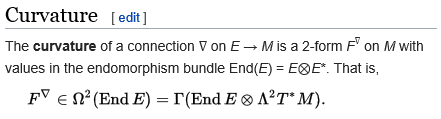
\includegraphics[width=11cm]{curvature_definition.png}

(from \url{https://en.wikipedia.org/wiki/Connection_(vector_bundle)}).

Here $\Gamma$ means `sections of', while you can set $E=TM$. Furthermore $\bigwedge^2 V$ is like $V \otimes V$ (but with additional rule that $v_1 \otimes v_2 = -v_2 \otimes v_1$ (as your first two friends can swap places)). Thus the text says that curvature is a section of the $T^* \otimes T^* \otimes T^* \otimes T$ bundle.

\end{frame}

\begin{frame}{Summary}

\begin{itemize}
\item{Definition of \textit{vector bundle} and of \textit{section}.}
\item{Bundles can be `twisted'; the topology can then place restrictions on the sections. This can arise even in simple settings (e.g. $TS^2$).}
\item{Derivative of a scalar function is a section of the cotangent bundle.}
\item{The central mathematical objects of GR are machines that act multi-linearly on tangent vectors to spacetime $M$. They are therefore sections of bundles that have been derived from $TM$.}
\end{itemize}

\end{frame}

\end{document}


